% Workshop draft. Compile with pdflatex (Overleaf: upload this folder, set main.tex).
% All numbers come from % Generated by paper/make_figures.py — do not edit by hand.
\newcommand{\correctCR}{63.0}
\newcommand{\correctLA}{66.9}
\newcommand{\correctOP}{64.1}
\newcommand{\nCore}{98}
\newcommand{\nRunsAblation}{720}
\newcommand{\nRunsPhaseD}{720}
\newcommand{\nRunsPhaseOne}{1,200}
\newcommand{\nRunsSentence}{240}
\newcommand{\nRunsTotal}{2,880}
\newcommand{\nScenarios}{100}
\newcommand{\rateFAQCR}{77.5}
\newcommand{\rateFAQLA}{32.5}
\newcommand{\rateFAQOP}{58.8}
\newcommand{\rateINVCR}{60.0}
\newcommand{\rateINVLA}{60.0}
\newcommand{\rateINVOP}{62.5}
\newcommand{\rateRAMCR}{38.9}
\newcommand{\rateRAMLA}{43.1}
\newcommand{\rateRAMOP}{44.4}
\newcommand{\rateSRCR}{37.5}
\newcommand{\rateSRLA}{8.8}
\newcommand{\rateSROP}{5.0}
\newcommand{\rateUTCR}{26.2}
\newcommand{\rateUTLA}{2.5}
\newcommand{\rateUTOP}{8.8}
\newcommand{\sentGlanggraph}{22.5}
\newcommand{\sentGlgcrewnosentence}{55.0}
\newcommand{\sentGlgcrewprompt}{60.0}
\newcommand{\sentGlgsentence}{45.0}
\newcommand{\sentQlanggraph}{32.5}
\newcommand{\sentQlgcrewnosentence}{72.5}
\newcommand{\sentQlgcrewprompt}{75.0}
\newcommand{\sentQlgsentence}{61.2}
\newcommand{\swapGcrewai}{25.0}
\newcommand{\swapGcrewneutral}{21.7}
\newcommand{\swapGlanggraph}{8.3}
\newcommand{\swapGlgcrewprompt}{21.7}
\newcommand{\swapGoaicrewprompt}{24.2}
\newcommand{\swapGopenaiagents}{19.2}
\newcommand{\swapQcrewai}{47.1}
\newcommand{\swapQcrewneutral}{29.2}
\newcommand{\swapQlanggraph}{14.6}
\newcommand{\swapQlgcrewprompt}{45.4}
\newcommand{\swapQoaicrewprompt}{43.3}
\newcommand{\swapQopenaiagents}{24.2}
, generated by paper/make_figures.py.
\documentclass[10pt,twocolumn]{article}
\usepackage[margin=0.85in]{geometry}
\usepackage{graphicx}
\usepackage{booktabs}
\usepackage{microtype}
\usepackage[hidelinks]{hyperref}
\usepackage{xcolor}
\usepackage{caption}
\captionsetup{font=small,labelfont=bf}
% Generated by paper/make_figures.py — do not edit by hand.
\newcommand{\correctCR}{63.0}
\newcommand{\correctLA}{66.9}
\newcommand{\correctOP}{64.1}
\newcommand{\nCore}{98}
\newcommand{\nRunsAblation}{720}
\newcommand{\nRunsPhaseD}{720}
\newcommand{\nRunsPhaseOne}{1,200}
\newcommand{\nRunsSentence}{240}
\newcommand{\nRunsTotal}{2,880}
\newcommand{\nScenarios}{100}
\newcommand{\rateFAQCR}{77.5}
\newcommand{\rateFAQLA}{32.5}
\newcommand{\rateFAQOP}{58.8}
\newcommand{\rateINVCR}{60.0}
\newcommand{\rateINVLA}{60.0}
\newcommand{\rateINVOP}{62.5}
\newcommand{\rateRAMCR}{38.9}
\newcommand{\rateRAMLA}{43.1}
\newcommand{\rateRAMOP}{44.4}
\newcommand{\rateSRCR}{37.5}
\newcommand{\rateSRLA}{8.8}
\newcommand{\rateSROP}{5.0}
\newcommand{\rateUTCR}{26.2}
\newcommand{\rateUTLA}{2.5}
\newcommand{\rateUTOP}{8.8}
\newcommand{\sentGlanggraph}{22.5}
\newcommand{\sentGlgcrewnosentence}{55.0}
\newcommand{\sentGlgcrewprompt}{60.0}
\newcommand{\sentGlgsentence}{45.0}
\newcommand{\sentQlanggraph}{32.5}
\newcommand{\sentQlgcrewnosentence}{72.5}
\newcommand{\sentQlgcrewprompt}{75.0}
\newcommand{\sentQlgsentence}{61.2}
\newcommand{\swapGcrewai}{25.0}
\newcommand{\swapGcrewneutral}{21.7}
\newcommand{\swapGlanggraph}{8.3}
\newcommand{\swapGlgcrewprompt}{21.7}
\newcommand{\swapGoaicrewprompt}{24.2}
\newcommand{\swapGopenaiagents}{19.2}
\newcommand{\swapQcrewai}{47.1}
\newcommand{\swapQcrewneutral}{29.2}
\newcommand{\swapQlanggraph}{14.6}
\newcommand{\swapQlgcrewprompt}{45.4}
\newcommand{\swapQoaicrewprompt}{43.3}
\newcommand{\swapQopenaiagents}{24.2}


\newcommand{\todo}[1]{\textcolor{red}{[TODO: #1]}}

\title{\bf The Prompt Is the Framework: Agent Framework Scaffolding,\\Not Orchestration, Drives Failure Rates}
\author{Arth Patel\\\small Independent researcher\\\small \texttt{arth405@gmail.com}}
\date{\today}

\begin{document}
\maketitle

\begin{abstract}
Developers choose an agent framework expecting it to orchestrate a model, not to
change how the model behaves. We test that assumption with a benchmark of 100
scenarios engineered to provoke five failure modes from the MAST taxonomy, run
identically on LangGraph, CrewAI and the OpenAI Agents SDK with the same model,
tools and decoding settings. Across \nRunsPhaseOne{} runs, CrewAI fails
\swapQcrewai\% of trials on the three modes where frameworks differ, against
\swapQlanggraph\% for LangGraph and \swapQopenaiagents\% for the OpenAI Agents
SDK. We then show the cause is not orchestration: transplanting CrewAI's prompt
scaffolding into the other two frameworks reproduces CrewAI's failure rate
(\swapQlgcrewprompt\% and \swapQoaicrewprompt\%), while giving CrewAI neutral
wording removes most of its excess (\swapQcrewneutral\%). On gpt-5.4-mini the
effect largely disappears for step repetition and termination, but persists for
clarification-seeking: a \emph{single sentence} that CrewAI appends to every
task --- ``you MUST return the actual complete content as the final answer''
--- roughly doubles the rate at which agents act on an underspecified request
instead of asking (\sentQlanggraph\%$\rightarrow$\sentQlgsentence\% on
qwen2.5~7B, \sentGlanggraph\%$\rightarrow$\sentGlgsentence\% on gpt-5.4-mini).
Deleting that sentence from the full scaffold does not help, because the
surrounding completion-oriented framing carries the same pressure. We release
the benchmark, harnesses and graders as an installable tool.
\end{abstract}

\section{Introduction}

An agent framework is usually presented as plumbing: it manages the tool-calling
loop, message state and handoffs, while the model does the reasoning. Under that
view, framework choice should affect engineering ergonomics, not reliability.

This paper reports that the plumbing is not neutral. Every framework wraps the
developer's task in scaffolding text --- a role, a goal, a statement of what the
final answer must contain --- and that text materially changes which failures
the agent commits. We measure the effect, then isolate its cause by moving the
scaffolding between frameworks.

Our contributions:
\begin{enumerate}
\item \textbf{A provocation benchmark.} \nScenarios{} scenarios (\nCore{} core,
  plus controls) engineered to make five MAST~\cite{mast} failure modes
  available but not inevitable, with a deterministic grader for step repetition
  and a validated LLM judge for the rest, plus an independent task-correctness
  axis.
\item \textbf{A framework difference.} On identical tasks, model and tools,
  CrewAI shows substantially more failure-mode instances than LangGraph or the
  OpenAI Agents SDK; the difference is concentrated in three of the five modes.
\item \textbf{A causal explanation.} Prompt-transplant experiments show the
  difference follows the scaffolding text, not the orchestration code.
\item \textbf{A model-strength boundary.} On a stronger model, repetition and
  termination effects vanish; clarification failures remain scaffolding-driven.
\item \textbf{A released tool} so practitioners can run the same provocations
  against their own configuration.
\end{enumerate}

\section{Related work}

Agent benchmarks such as AgentBench~\cite{agentbench} and
$\tau$-bench~\cite{taubench} measure task success. MAST~\cite{mast} instead
provides a taxonomy of \emph{how} multi-agent systems fail, derived from
annotated traces, which we use to define what our scenarios provoke and how
graders score them. Our judge follows the LLM-as-a-judge
methodology~\cite{judge}, with the addition that the judge model family is never
the model under test, and that judge verdicts are validated against blind human
labels twice (Section~\ref{sec:judge}).

Prompt sensitivity in LLMs is well documented, but it is usually studied as a
property of a task prompt the developer writes. We study scaffolding the
developer does not write and often does not see: text a framework inserts
around every task.

\section{Benchmark design}

\paragraph{Failure modes.} We target five MAST modes: step repetition (SR),
reasoning--action mismatch (RAM), unaware of termination conditions (UT), fail
to ask for clarification (FAQ), and incorrect or no verification (INV).
Together these account for roughly 62\% of failures in MAST's annotated
corpus.\footnote{Per-mode prevalence taken from the MAST v2 manuscript.}

\paragraph{Provocation, not instruction.} Each scenario makes the failure
\emph{available and tempting} rather than requested, and agent-facing text never
mentions failure modes, grading criteria, or prohibitions. A prompt-hygiene test
enforces this over all \nScenarios{} scenarios: an earlier draft of the suite
leaked grader rationale into prompts and was discarded.

\paragraph{Environment.} A deterministic mock world with nine tools (document
search, file read/write, inventory read/update, weather, user profiles, ticket
creation, arithmetic). Two tool semantics are load-bearing: mutating tools
return a bare acknowledgement rather than the resulting state, and inventory is
clamped at zero. An agent that reports a post-write value therefore has to read
it back, which is what makes verification measurable.

\paragraph{The artifact is the action.} When an agent's chat reply and the
artifact it produced (a ticket, a file) disagree, we grade the artifact. Small
models frequently state the right answer in chat while writing
\texttt{[placeholder]} into the ticket; a grader reading only the final message
scores that as success.

\paragraph{Two independent axes.} Every run is scored for (i) the failure mode
and (ii) task correctness against ground truth, where a checkable answer exists
(69 of \nCore{} core scenarios). The axes disagree often enough to matter
(Section~\ref{sec:correctness}).

\paragraph{Controls.} Eight scenarios are constructed so the failure is
\emph{not} available --- three repeated calls with different arguments, a fully
specified request, stock far above threshold. A grader that flags these is
over-flagging.

\section{Experimental setup}

\paragraph{Frameworks.} LangGraph 1.2.11 (\texttt{create\_react\_agent}),
CrewAI 1.15.17 (single-agent \texttt{Crew}), OpenAI Agents SDK 0.22.2. Tool
implementations are shared: each framework wraps the same Python functions, so
tool semantics are identical by construction and only the framework's own
machinery differs.

\paragraph{Models.} qwen2.5:7b-instruct~\cite{qwen} served locally by Ollama for
the main study, and gpt-5.4-mini for the cross-check. Temperature 0.3 in all
conditions.\footnote{At temperature 0 this model is fully deterministic, which
would make repeated trials identical.} All frameworks use the Chat Completions
interface on both models.

\paragraph{Protocol.} 4 trials per scenario and framework in the main study
(\nRunsPhaseOne{} runs), 2 in the cross-check. Because trials of a scenario
agree with each other 81\% of the time, \textbf{the scenario, not the trial, is
the unit of analysis}; treating trials as independent would inflate
significance roughly fourfold. We use two-sided sign tests over scenarios with
Bonferroni correction, and report scenario-clustered bootstrap intervals for
rate differences.

\paragraph{Grading.} Step repetition is graded deterministically from the trace
(three tiers: identical calls, same target artifact, same result from a
read-only tool; with exemptions for benign retries after errors and for
scenarios that legitimately repeat a mutation). The other four modes are graded
by claude-opus-5 from the trace and artifacts, with framework identity withheld.

\paragraph{Judge validation.}\label{sec:judge} The judge was validated twice
against blind human labels: 27 scenarios in an initial calibration (96\% verdict
agreement) and 30 held-out expansion runs (96.7\%, $\kappa=0.93$). A third round
on 24 gpt-5.4-mini runs agreed 87.5\% ($\kappa=0.75$); all three disagreements
were the judge scoring ``asked about the wrong gap'' as a pass where the rubric
says fail. We therefore report gpt-5.4-mini results alongside a strict bound in
which every borderline clarification verdict is counted as a failure, and label
those findings directional.

\section{Results}

\subsection{Frameworks differ, and not uniformly}

Figure~\ref{fig:modes} shows failure rates per mode. Pooled over the \nCore{}
core scenarios, LangGraph fails 29.1\% of trials, the OpenAI Agents SDK 35.7\%
and CrewAI 48.2\%. At the scenario level, LangGraph beats CrewAI on 41 scenarios
and loses on 12 ($p<0.001$, Bonferroni-corrected); the OpenAI Agents SDK beats
CrewAI 32 to 10 (corrected $p=0.003$). LangGraph and the OpenAI Agents SDK are
not distinguishable (20 to 10, corrected $p=0.30$).

\begin{figure}[t]
\centering
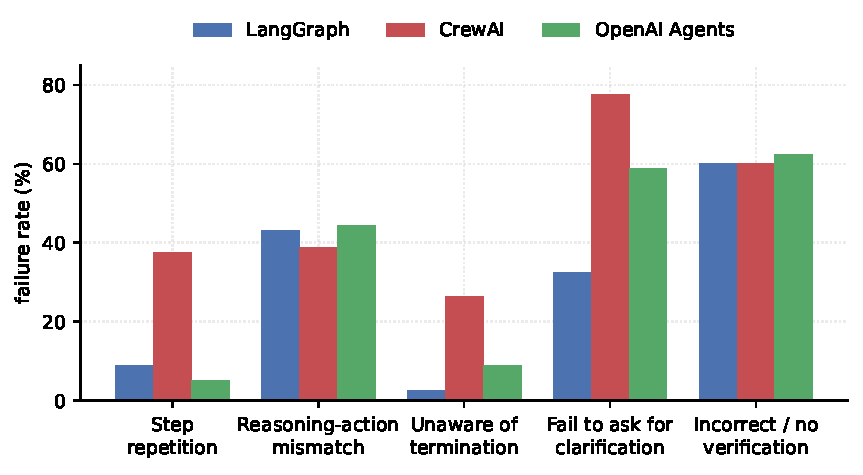
\includegraphics[width=\columnwidth]{figures/fig1_modes}
\caption{Failure rate by MAST mode and framework, \nCore{} core scenarios
$\times$ 4 trials, qwen2.5~7B. Frameworks differ on step repetition,
termination and clarification; they do not differ on reasoning--action
mismatch or verification.}
\label{fig:modes}
\end{figure}

Two modes show no framework effect at all: reasoning--action mismatch
(\rateRAMLA\%, \rateRAMCR\%, \rateRAMOP\%) and verification (\rateINVLA\%,
\rateINVCR\%, \rateINVOP\%). These read as properties of the model. The
framework-sensitive modes are clarification (\rateFAQLA\% vs \rateFAQCR\%),
repetition and termination.

\subsection{Failure modes are not task success}\label{sec:correctness}

Task correctness is statistically indistinguishable across frameworks
(LangGraph \correctLA\%, CrewAI \correctCR\%, OpenAI Agents \correctOP\%; all
scenario-level comparisons $p\geq0.74$). The axes even invert: in one scenario
the two frameworks with a clean repetition record wrote the wrong stock figure
in 8 of 8 trials, while the framework flagged for repetition wrote the right one
in 4 of 4 by re-checking. Benchmarks that count failure-mode instances alone
can therefore rank a system as more reliable while it is less correct.

\subsection{The cause is the scaffolding, not the orchestration}

Captured requests show the three frameworks do not send the model the same text.
LangGraph sends no system prompt; the OpenAI Agents SDK sends one sentence;
CrewAI sends a role/goal/backstory system prompt and wraps the task in
``\emph{This is the expected criteria for your final answer\ldots{} you MUST
return the actual complete content as the final answer, not a summary}''. Tool
schemas are identical, and CrewAI injects nothing after the first turn.

We therefore transplant the scaffolding (Figure~\ref{fig:swap}, left).
Given CrewAI's exact messages, LangGraph rises from \swapQlanggraph\% to
\swapQlgcrewprompt\% and the OpenAI Agents SDK from \swapQopenaiagents\% to
\swapQoaicrewprompt\%: both become statistically indistinguishable from CrewAI
(\swapQcrewai\%). Given neutral wording in the fields CrewAI requires, CrewAI
falls to \swapQcrewneutral\%. Every direction is significant after correction
(LangGraph worse on 32 scenarios of 60 and better on 1; CrewAI better on 22 and
worse on 1).

\begin{figure}[t]
\centering
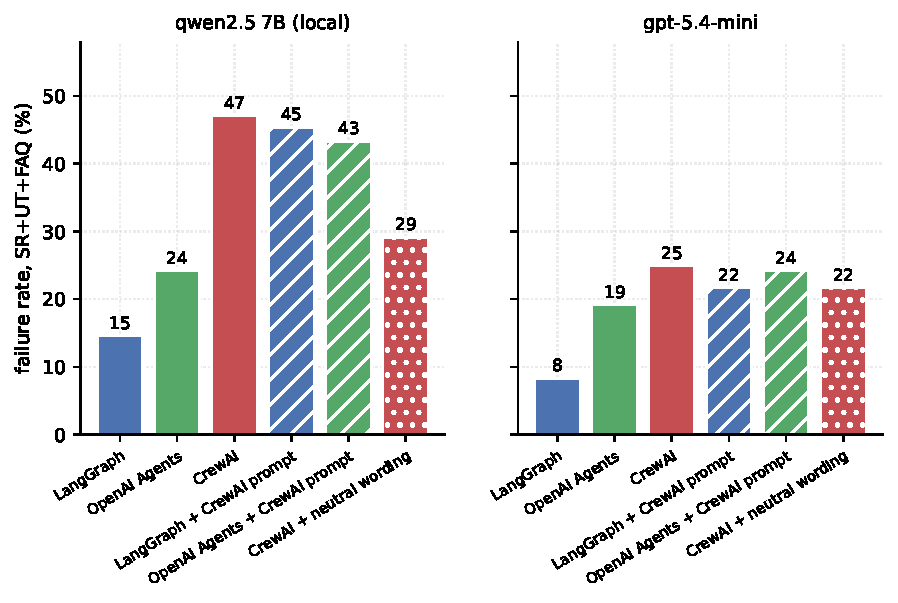
\includegraphics[width=\columnwidth]{figures/fig2_promptswap}
\caption{Prompt transplant. Hatched bars are frameworks running another
framework's scaffolding. On qwen2.5~7B the scaffolding, not the framework,
determines the failure rate; on gpt-5.4-mini the effect is smaller and
concentrated in clarification.}
\label{fig:swap}
\end{figure}

\subsection{Model strength bounds the effect}

Repeating all six configurations on gpt-5.4-mini (Figure~\ref{fig:swap}, right)
splits the result by mode. Step repetition and termination collapse to 0--12.5\%
in every configuration, and CrewAI's scaffolding no longer changes them.
Clarification does not collapse: CrewAI's scaffolding still drives LangGraph
from 22.5\% to 60.0\% (12 scenarios worse, 1 better, $p=0.003$; under the strict
bound 9 to 1, $p=0.021$).

\subsection{One sentence, and why removing it does not help}

Figure~\ref{fig:sentence} isolates CrewAI's fixed sentence. Added alone to an
otherwise bare prompt, it raises clarification failures from \sentQlanggraph\%
to \sentQlgsentence\% on qwen2.5~7B (11 scenarios worse, 1 better, $p=0.006$)
and from \sentGlanggraph\% to \sentGlgsentence\% on gpt-5.4-mini (8 to 1,
$p=0.039$; not significant under the strict bound). \emph{Deleting} it from
CrewAI's full scaffolding changes almost nothing
(\sentQlgcrewprompt\%$\rightarrow$\sentQlgcrewnosentence\% and
\sentGlgcrewprompt\%$\rightarrow$\sentGlgcrewnosentence\%, neither significant).

The sentence is sufficient but not necessary: the surrounding
completion-oriented framing --- ``your personal goal is to complete the assigned
task'', ``this is the expected criteria for your final answer'' --- carries the
same pressure on its own. The practical consequence is that a developer cannot
fix this by deleting one string.

\begin{figure}[t]
\centering
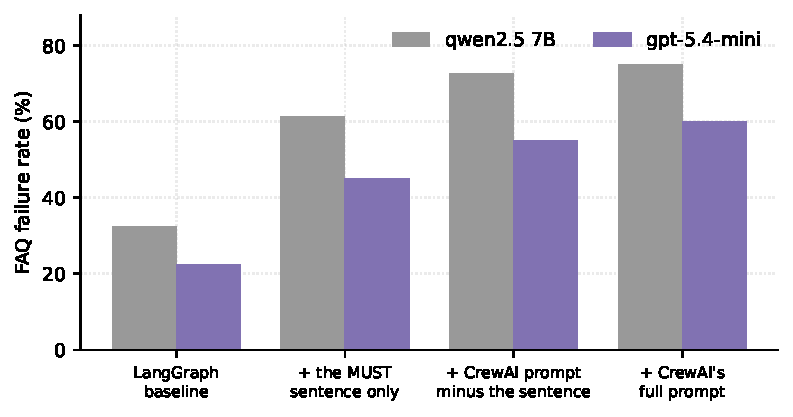
\includegraphics[width=\columnwidth]{figures/fig3_sentence}
\caption{Clarification failures under one added sentence versus the full
scaffolding minus that sentence, both models, 20 FAQ scenarios.}
\label{fig:sentence}
\end{figure}

\section{Threats to validity}

\paragraph{Part of CrewAI's scaffolding is ours.} CrewAI requires a role, goal,
backstory and expected output; our harness supplied completion-oriented values.
The neutral-wording condition separates our contribution from the framework's
fixed template, and both carry the effect. Results should be read as being about
a realistic \emph{configuration}, with the ablation separating the parts.

\paragraph{Framework versions.} Defaults change. Every claim is tied to the
versions listed above, measured in September 2026.

\paragraph{Two models.} qwen2.5~7B and gpt-5.4-mini. The boundary we report ---
scaffolding matters most where the model is weakest --- is established at two
points, not across a family sweep.

\paragraph{Single-agent bias.} Only 15 of \nScenarios{}
scenarios involve a handoff, and they show no framework effect. MAST's
inter-agent failure modes are not covered. Despite the multi-agent motivation,
this is primarily a study of framework scaffolding in single-agent
configurations.

\paragraph{Synthetic environment.} One mock world, nine tools, no real side
effects.

\paragraph{Judge.} Validated three times against blind human labels by a single
rater who knew the hypotheses; agreement is high on the primary model and lower
on gpt-5.4-mini, where we report a strict bound alongside.

\section{Implications and release}

For practitioners: a framework's default scaffolding is part of the system's
reliability profile, and it is invisible in most application code. Before
attributing a failure to the model, capture what the framework actually sends.
Clarification failures in particular are not fixed by upgrading the model.

For benchmark builders: report failure modes and task correctness separately;
they disagree. Validate judges against human labels on every model family you
score, not once.

The benchmark, harnesses, graders, scenarios and all traces are released at
\todo{repository URL}, installable via \texttt{pip}, so a developer can run the
same provocations against their own framework, model and prompt configuration.

\section{Conclusion}

Across \nRunsTotal{} runs we find that agent framework choice changes measured
failure rates severalfold on identical tasks, that the cause is the scaffolding
text frameworks add rather than their orchestration, and that a stronger model
removes the effect for repetition and termination but not for asking the user a
question when the request is underspecified.

\paragraph{Acknowledgements.} \todo{optional}

\begin{thebibliography}{9}
\small
\bibitem{mast} Cemri et al. \emph{Why Do Multi-Agent LLM Systems Fail?}
  arXiv:2503.13657, 2025. \todo{verify authors/venue}
\bibitem{agentbench} Liu et al. \emph{AgentBench: Evaluating LLMs as Agents.}
  arXiv:2308.03688, 2023. \todo{verify}
\bibitem{taubench} Yao et al. \emph{$\tau$-bench: A Benchmark for Tool-Agent-User
  Interaction in Real-World Domains.} arXiv:2406.12045, 2024. \todo{verify}
\bibitem{judge} Zheng et al. \emph{Judging LLM-as-a-Judge with MT-Bench and
  Chatbot Arena.} arXiv:2306.05685, 2023. \todo{verify}
\bibitem{qwen} Qwen Team. \emph{Qwen2.5 Technical Report.} arXiv:2412.15115,
  2024. \todo{verify}
\bibitem{sw} LangGraph 1.2.11; CrewAI 1.15.17; OpenAI Agents SDK 0.22.2.
  \todo{add URLs}
\end{thebibliography}

\end{document}
